
\chapter{\JV System}
\label{chap:system}

This chapter discusses the \JV system. We present a high level view of the
system, supported changes, and the \JV Virtual Machine implementation.

\begin{figure}[t]
\centering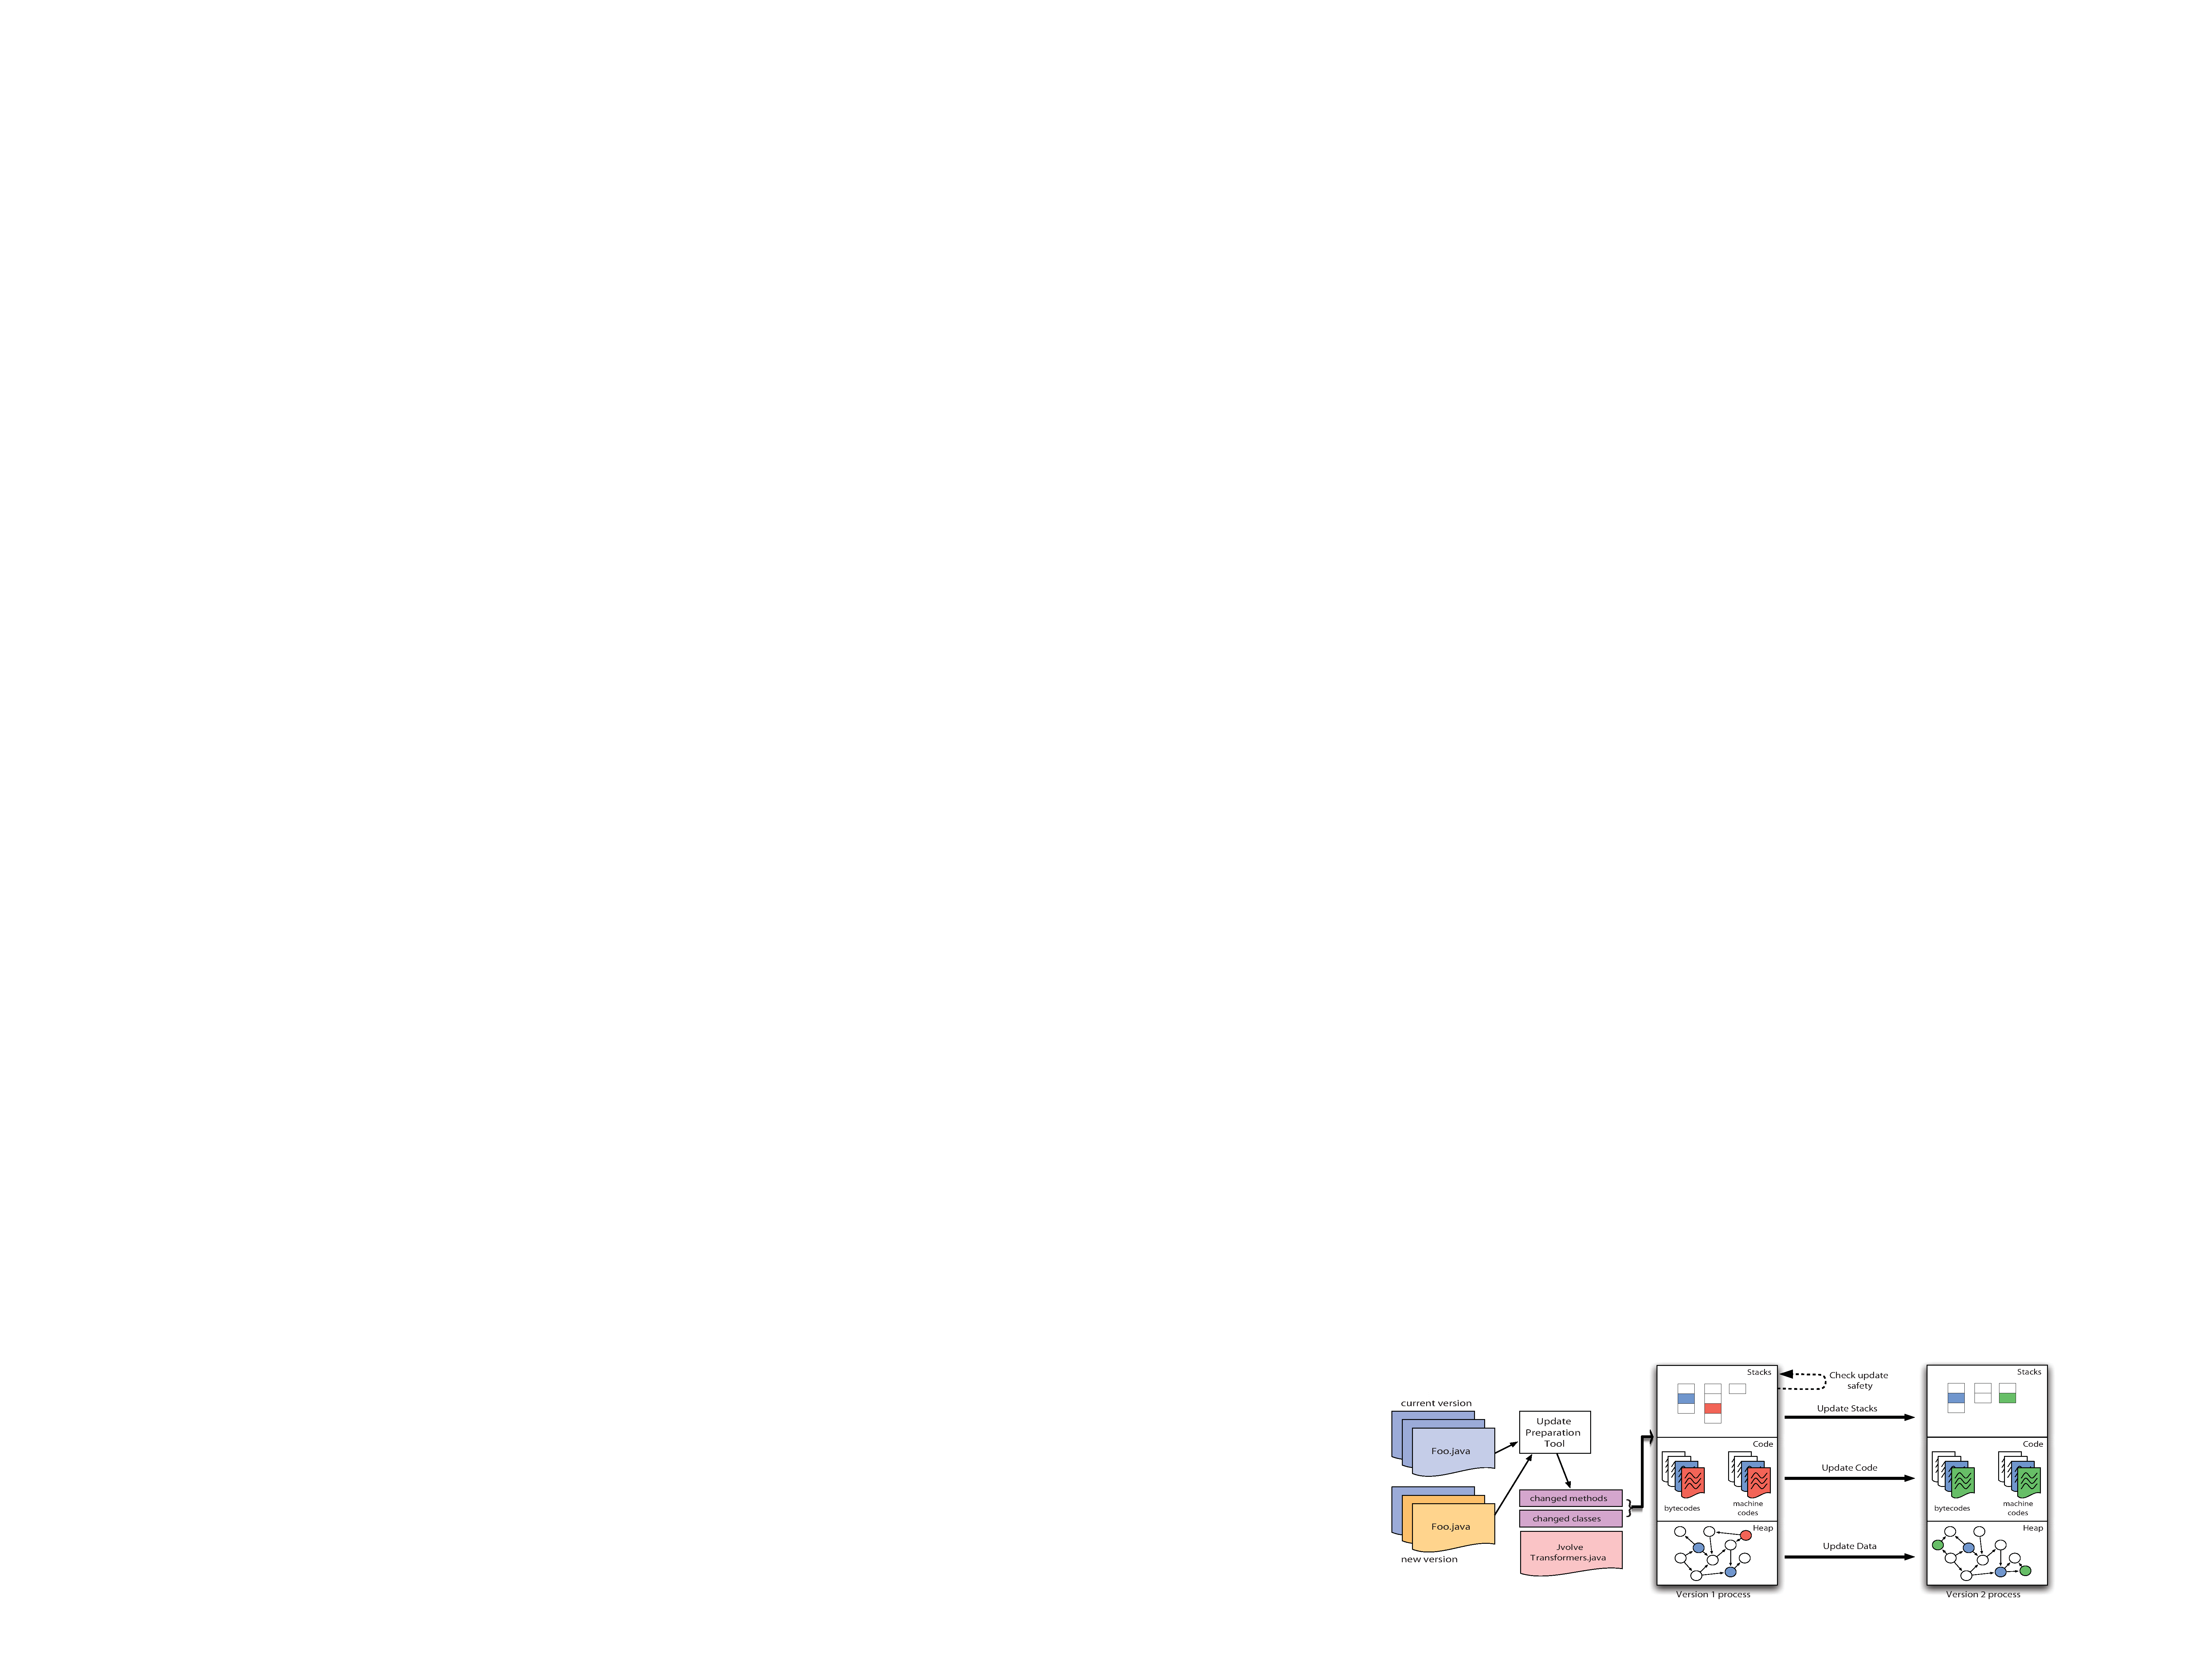
\includegraphics[scale=0.38,clip=true,trim=2170 90 250 2125]{100-images/PASS-HPC-poster-8-2009-cropped}
\caption{Overview of the Dynamic Updating process.\label{fig:overview}}
\end{figure}

\section{Introduction}
\label{sec:system-intro}

Figure~\ref{fig:overview} illustrates the dynamic updating process. The left
portion depicts the work done offline. The developer writes the old and new
versions of the application, and tests them as part of the software
development process. The \acf{UPT} examines source code
of the old and new versions of the application and prepares a dynamic patch.
The user feeds the patch to a process with dynamic-updating support,
depicted on the right. The figure shows two processes, one
running version one of an application, showing stacks, code and heap; and
another running version two of the same application. The goal is to
transition from a process running an old version of the application, to one
running the new version, on the fly, without stopping and restarting the
application.

We assume that developers write and fully test both the old and new
versions using standard development practices without anticipating that
the application is going to be updated dynamically. Testing is already a
well established part of software development. With dynamic updating,
developers should test the update process, in addition to testing their
applications.
When it comes time to
perform the update, the developer provides the source code for the old and
new versions to \JV's \acf{UPT}. The \acs{UPT} compares these two versions
and provides a specification for the update. The specification consists of
two major parts. First, it contains information about code changes that
inform the VM when it is safe to perform the update, what old
methods to invalidate, and what new method bodies to load. Second, it
informs the VM how to deal with changes to data. The VM uses this
specification to transform classes and objects in the heap to conform to
their new version. The programmer has the option to
modify the update specification. Specifically, the
\acs{UPT} does not reason deeply about the semantics of
data structure changes. The programmer may need to modify the \acs{UPT}s
output to obtain a correct program.

Given an update specification, the user
signals the running VM to apply the update.  The VM loads the new class
files and schedules the update. The VM scheduler signals an interrupt, which
stops all threads at VM safe points, where it is safe to perform thread
scheduling and garbage collection. \JV then checks if the VM is at a
\emph{DSU safe point}. DSU safe points require that no thread's activation
stack contains a \emph{restricted} method, which is part of the specification.

Restricted methods are of three categories: (1) methods changed by the
update, (2) methods whose bytecode is unchanged but whose compiled
representation may change, and (3) methods specified by the user or
testing process for semantic reasons. If
restricted methods are on stack, the VM installs return-barriers for~(1)
and~(3), and performs on-stack-replacement for~(2) to reach a DSU safe
point.  Section~\ref{sec:safe} describes how \JV reaches a safe point in
detail.

Once all application threads have synchronized at DSU safe points, \JV
applies the update. It first invalidates the compiled versions of all
changed methods.  These methods are recompiled as needed---the adaptive JIT
compiler will generate code the next time the program invokes an
invalidated method, and will optimize it further, if the program executes it
frequently enough.  The VM then initiates a full copying garbage collection. It
piggybacks on the garbage collector to detect all existing objects whose
classes change. It allocates objects that conform to the new class
definitions.
Finally, after garbage collection, \JV performs class and
object transformations to populate per-class static fields and per-object
instance fields with valid state.  At this point, the update is complete.

\section{Supported Changes}
\label{sec:supported-changes}

We have designed a simple, yet flexible update model that supports updates
that we have seen to be common in practice.

\paragraph{Method body changes}
Programmers may change method bodies. Method body updates are the simplest
and most commonly supported change~\cite{JVMhotswap, VSEnC, eaddy05enc,
GilmoreKW97, orso:java, K42reconfig, HjalmtyssonG98}. DSU systems
can preserve type safety by simply invoking the new method the next time
the program executes the method. However, restricting updates to only method
bodies prevents many common changes~\cite{neamtiu05evolution}.
Chapter~\ref{chap:experience} shows that over half the releases of Jetty,
JavaEmailServer, and CrossFTP, the programs we studied, change more than method bodies.

\paragraph{Class signature changes}
Programmers may also change class signatures in various ways.
% By class signature, we mean the interface a class exposes to other classes and
% methods.
The class signature includes all fields and methods defined by the class
and those inherited from super classes. A programmer may change method
signatures by changing the type or number of method arguments. They
may add or delete virtual and static field members, and change the types or
access modifiers of existing members.  These changes may occur at any level
of the class hierarchy.  For example, programmers may delete a field from a
parent class and this change will propagate correctly to the class's
descendants.
% We rely on the bytecode compiler to ensure that the resulting
% program is type-safe, and thus there are no more accesses to the deleted field
% in the program.  

\begin{figure}[t]
\begin{tabular}{@{}m{0.5\textwidth}@{}m{0.5\textwidth}@{}}
\BC \begin{minipage}{0.4\textwidth}
\begin{lstlisting}
private int x;
private static int y;
public int getX();
public static int getY();
\end{lstlisting}
\end{minipage} \EC &
\BC \begin{minipage}{0.45\textwidth}
\begin{lstlisting}
private double x;
private static double y;
public double getX();
public static double getY();
\end{lstlisting}
\end{minipage} \EC \\[-2ex]
\BC (a) Old version \EC &
\BC (b) New version \EC \\[-2ex]
\end{tabular}
\caption{Examples of an update that changes class signature}
\label{fig:class-sig-change-example}
\end{figure}


\begin{figure}[p]
\BC \begin{minipage}{0.92\textwidth}
\begin{lstlisting}[frame=single]
public class User {
  private final String username, domain, password;
  private String[] forwardAddresses;
  public User(...) {...}
  public String[] getForwardedAddresses() {...}
  public void setForwardedAddresses(String[] f) {...}
}
public class ConfigurationManager {
  private User loadUser(...) {
     ...
     User user = new User(...);
     String[] f = ...;
     user.setForwardedAddresses(f);
     return user;
  }
}
\end{lstlisting}
\end{minipage} \\
(a) Version 1.3.1 \EC

\BC \begin{minipage}{0.92\textwidth}
\begin{lstlisting}[frame=single]
public class User {
  private final String username, domain, password;
  private EmailAddress[] forwardAddresses;
  public User(...) {...}
  public EmailAddress[] getForwardedAddresses() {...}
  public void setForwardedAddresses(EmailAddress[] f) {...}
}
public class ConfigurationManager {
  private User loadUser(...) {
     ...
     User user = new User(...);
     EmailAddress[] f = ...;
     user.setForwardedAddresses(f);
     return user;
  }
}
\end{lstlisting}
\end{minipage} \\
(b) Version 1.3.2 \EC
\hangcaption{Changes to JavaEmailServer \User and {\tt
ConfigurationManager} classes from version 1.3.1 to version 1.3.2}
\label{fig:jes-string-emailaddress-example}
\end{figure}


Figure~\ref{fig:class-sig-change-example} provides examples of class
signature changes. Each line in the figure defines either a field or a
method and represents a class signature change in the new version.
Internally, \UPT does not view this update as changing the signature of
individual fields and methods. Instead, it views the update as removing the
field {\tt int x} and adding a new field {\tt double x}, and similarly for
the methods. Irrespective of how \UPT views this change, it is pertinent to
note that any reference to these fields and methods in the new version must
conform to the new type signature. The Java to bytecode compiler
will ensure that the standalone new version of the program is well-formed.

\JV does not support permutations of the class hierarchy, e.g., reversing
a super-class relationship.  While this change may be desirable in
principle, in practice, it requires sophisticated transformers that enforce
update ordering constraints. None of the program versions we examined make
this type of change. \JV also does not support renaming a class, though
this functionality should be easy to add.
% While it
% is not hard to implement this support, we did not 

% In summary, \UPT recognizes changes with method bodies and changes that add
% or remove fields or methods.

\paragraph{Example.} Consider the following update from JavaEmailServer, a
simple SMTP and POP e-mail server.
Figure~\ref{fig:jes-string-emailaddress-example} illustrates a pair of
classes that change between versions 1.3.1 and 1.3.2.  \JV fully supports
these changes. JavaEmailServer uses the class \User to maintain information
about e-mail user accounts in the server.  Moving from version 1.3.1 to
1.3.2, there are three differences. First, the method {\tt loadUser} fixes
some problems with the loading of forwarded addresses from a configuration
file (details not shown). This change is a simple method update.  Second,
the array of forwarded addresses in the new version contains instances of a
new class, {\tt EmailAddress}, rather than {\tt String}.  This change
modifies the class signature of \User since it modifies the type of {\tt
forwardedAddresses}. Finally, the class's {\tt setForwardedAddresses}
method is also altered to take an array of {\tt EmailAddress}es instead of
an array of {\tt String}s, and code from {\tt loadUser} accommodates this
change as well.

\section{VM object model and method dispatch}
\label{sec:dsu-view-of-changes}
\JV's dynamic application of an update closely follows \UPT's static specification, and
is related to how a
\JVM would support field accesses and method calls. In
languages such as C and Java accessing a field involves reading to or
writing from an offset from a structure or object's address. This offset is
determined at compile-time. In a language like Java, by compile-time we
mean the time when bytecode is translated to machine code. Method calls in
C, involve jumping to a memory location that contains the machine code for
the called method. Method calls in Java are similar, except that a \JVM
needs to support \emph{virtual method dispatch}. There can be different
definitions of the same method and which one is invoked depends on the
object in hand. \JVM{}s use \aclp{VMT} which contain pointers to compiled
machine codes of methods. A method call looks up the contents of a particular
slot in the \VMT and jumps to that address.

\begin{figure}[p]
\lstset{frame=single}
\begin{tabular}[t]{@{}c@{ }c@{}}
\begin{minipage}{0.35\textwidth}
\begin{lstlisting}
public class A {
  private int x, y;
  public void f() {
    g();
  };
  public void g() {
    this.y = 0;
  }
}

public class B
          extends A {
  private int z;
  public void g() {
    this.z = 0;
  }
  public void h() {}
}
\end{lstlisting}
\end{minipage}
&
\begin{minipage}{0.64\textwidth}
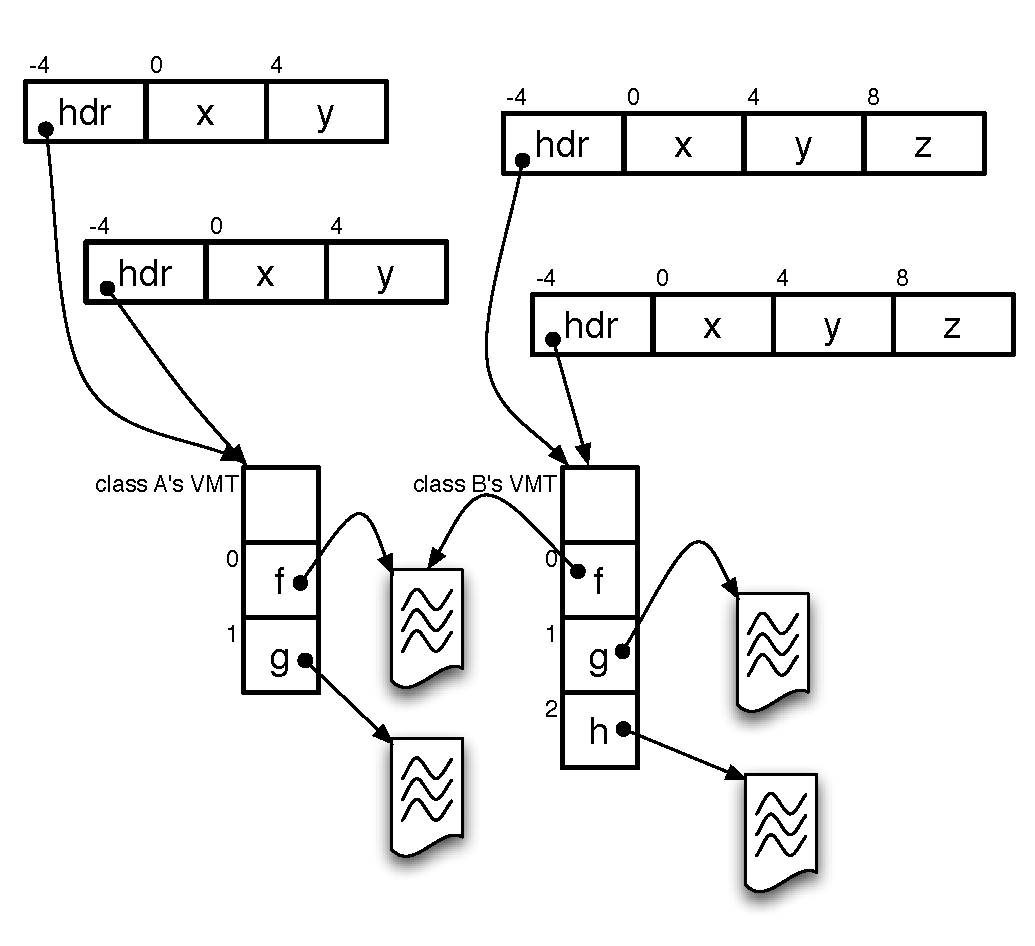
\includegraphics[draft=false,scale=0.5]{100-images/field-method-access-explanation}
\end{minipage} \\
\begin{minipage}{0.28\textwidth}
(a) Java source code
\end{minipage} &
\begin{minipage}{0.44\textwidth}
(b) Objects and VMTs in the heap
\end{minipage} \\[2ex]
\begin{minipage}{0.35\textwidth}
\begin{lstlisting}
aload_0
invokevirtual <A.g>
return
\end{lstlisting}
\vspace{-2ex}
\BC (a) Bytecode for A.f() \EC
\end{minipage} &
\begin{minipage}{0.55\textwidth}
\lstset{moredelim=[il][commentstyle]{>}}
\begin{lstlisting}
>The stack pointer points to "this"
>EDX := this
        MOV     EDX      [ESP]
>The VMT is at offset -4
>ECS := VMT
        MOV     ECX   -4[EDX]
>Send this parameter in EAX
>EAX := this
        MOV     EAX      [ESP]
>Call function g()
>g() is at offset 8 within VMT
        CALL 8[ECX]
\end{lstlisting}
\end{minipage} \\
% \begin{minipage}{0.28\textwidth}
% (c) Bytecode for A.f()
% \end{minipage} &
&
\begin{minipage}{0.38\textwidth}
(d) Machine code for the {\tt invokevirtual} instruction
\end{minipage} \\
\end{tabular}
\hangcaption{Simple example of method and field accesses to illustrate how
inheritance is implemented in Java}
\label{fig:field-method-access-explanation}
\lstset{frame=none}
\end{figure}


We illustrate how a typical VM supports field accesses and method calls
with a simple example shown in
Figure~\ref{fig:field-method-access-explanation}. The class {\tt A} defines two
integer fields {\tt x} and {\tt y}. Objects of type {\tt A} have these
fields laid out contiguously. Objects of {\tt class B} have an additional
integer field {\tt z}. In managed languages, the runtime system maintains a header
field for all objects, which it uses to look up at runtime the type of a particular
object instance. The runtime also uses the object header to look up the
type's \VMT to invoke methods.
{\tt class A}'s
\VMT has method {\tt f()} at slot 0 and method {\tt g()} at slot 1. The
class
{\tt B} overrides method {\tt g()}. In addition, {\tt class B} defines a
new method {\tt h()} that takes slot 2.
Figure~\ref{fig:field-method-access-explanation}~(b) shows
\VMT{}s of {\tt A} and {\tt B}. \VMT slots point to compiled machine code
of respective methods. {\tt A.f()} and {\tt B.f()} both point to the same
code, while {\tt A.g()} and {\tt B.g()} point to different methods since
{\tt B} overrides {\tt g()}. The figure also shows objects of type {\tt A} and
{\tt B}.  The header field of these objects (chosen arbitrarily to be
at offset -4) allow access to their respective \VMT{}s.

Figure~\ref{fig:field-method-access-explanation}~(d) shows function {\tt
f()}'s generated machine code. The call to {\tt g()} refers to \VMT slot 1
(at offset 8). This call invokes either {\tt A.g()} or {\tt B.g()} based on
the type of the object making the call.  Whenever the \VMT slot of a method
is known at compile time, callers of that method use the offset in their
machine code. Similarly, the machine code usually contains offsets of
fields as well --- for instance, functions {\tt A.g()} and {\tt B.g()}
referring to offsets for {\tt y} and {\tt z} respectively. The interface a \VM
presents to the compiler consists of the following --- \acl{VMT} with methods
at various slots, and objects with fields laid out at various offsets.

\section{\JV's view of updates}

\JV groups updates presented by the \UPT into two categories --- those that
change the exposed representation of a class, and those that don't. \JV
handles updates as follows.
\begin{itemize}
\item Method body changes: \JV invalidates any old machine code, loads the
new bytecode of the method, and lazily generates new machine code.
\item Class signature changes:
  \begin{enumerate}
  \item The update changes the number and offsets of fields within an object. \JV creates
        new object instances that conform to the layout of the new version
        and copies fields appropriately. \JV also needs to initialize
        fields that do not exist in the old version.
        Section~\ref{subsec:transformers}
        talks about such changes and how \JV transforms objects to conform
        to the semantics of the application.
  \item The update changes the number and offsets of method slots in a class' \acl{VMT}. \JV
        creates new \VMT{}s and points all object instances to this new \VMT.
  \end{enumerate}
\item Methods that are not changed by the update but that refer to classes
with signature changes. The machine code of such methods will have field
and method offsets that are invalid in the new version. \JV invalidates old
codes, and lazily recompiles
such methods to generate machine code afresh. We refer to such methods as
\emph{indirect updates}.
\end{itemize}

\JV, with respect to the implementation of dynamic updating, does not view
classes as monolithic collections of fields and methods. Instead it views
them as method bodies that need to be updated, and structure instances
whose fields need to be aligned and have proper values to conform to the
semantics of the new version.

\subsection{Class and Object Transformers}
\label{subsec:transformers}

For classes whose signatures have changed, an object
transformer\index{object transformer} method  initializes a new version of
the object based on the old version. For example, consider the class
{\tt Point} in Figure~\ref{fig:point}. The {\tt Point} class in the old
version represents points in a 2-dimensional space with fields {\tt x} and
{\tt y}. After the update, the new version represents points in a
3-dimensional space with the additional field {\tt z}. The object transformer's
job is to modify each object instance of type {\tt Point} in the heap to conform to its
new class definition. Class transformers serve a similar purpose and update
static fields, rather than instance fields.  The \ac{UPT} generates default
class and object transformers automatically, retaining unchanged fields and
initializing new or changed ones.  The default object transformer, show in
Figure~\ref{fig:point}~(c)  for our changed \texttt{Point} class copies
fields {\tt x} and {\tt y} from an old object to a transformed object and
initializes {\tt z} to zero.

\begin{figure}[t]
\lstset{frame=single}
\begin{tabular}{@{}m{0.5\textwidth}@{}m{0.5\textwidth}@{}}
\BC \begin{minipage}{0.25\textwidth}
\begin{lstlisting}
class Point {
  double x, y;
}
\end{lstlisting}
\end{minipage} \EC &
\BC \begin{minipage}{0.29\textwidth}
\begin{lstlisting}
class Point {
  double x, y, z;
}
\end{lstlisting}
\end{minipage} \EC \\[-2ex]
\BC (a) Old version \EC &
\BC (b) New version \EC \\[-2ex]
\end{tabular}
\centering\begin{minipage}{0.55\textwidth}
\begin{lstlisting}
class JvolveTransformers {
  public static void jvolveObject(
    Point to, old_Point from) {
    to.x = from.x;
    to.y = from.y;
    to.z = 0.0;
  }
}
\end{lstlisting}
(c) Default UPT-generated object transformer
\end{minipage}
\caption{Example of a simple class and the default object transformer}
\label{fig:point}
\lstset{frame=none}
\end{figure}


% For example, consider a class \texttt{List} with field
% \texttt{next} of type \texttt{List} and an update that adds a new
% \texttt{int} field {\tt x} to \texttt{List}. The object transformer's
% job is to modify each object instance of type \texttt{List} to conform
% to its new class definition. Class transformers serve a similar
% purpose and update static fields, rather than instance
% fields.  The \ac{UPT} generates default class and object transformers
% automatically, retaining unchanged fields and initializing new or
% changed ones.  The default object transformer for our changed
% \texttt{List} copies the \texttt{next} field from an old object to a
% transformed object and initializes {\tt x} to zero, i.e,
% \texttt{transformed.next = old.next} and \texttt{transformed.x = 0}.

\begin{figure}[t]
\centering
\begin{minipage}{0.9\textwidth}
\begin{lstlisting}[frame=single]
public class v131_User {
  private final String username, domain, password;
  private String[] forwardAddresses;
}
public class JvolveTransformers {
 ...
 public static void jvolveClass(User unused) {}
 public static void jvolveObject(User to, v131_User from) {
    to.username = from.username;
    to.domain = from.domain;
    to.password = from.password;
    // default transformer would have:
    //   to.forwardAddresses = null
    int len = from.forwardAddresses.length;
    to.forwardAddresses = new EmailAddress[len];
    for (int i = 0; i < len; i++) {
      String[] parts =
        from.forwardAddresses[i].split("@", 2);
      to.forwardAddresses[i] =
        new EmailAddress(parts[0], parts[1]);
    }
  }
}
\end{lstlisting}
\end{minipage}
\hangcaption{\User object transformer for update from JavaEmailServer version
1.3.1 to version 1.3.2}
\label{fig:jes-transformer-code}
\VspaceFixForHangcaption
\end{figure}


For our example from JavaEmailServer in
Figure~\ref{fig:jes-string-emailaddress-example}, the \UPT identifies that
the \User and {\tt ConfigurationManager} classes have changed, and produces
default object transformers.  The programmer elects to modify the object
transformer for the class \User, as illustrated in
Figure~\ref{fig:jes-transformer-code}.
  
Object and class transformer methods are simply \static methods in the
class \JT, which is created by \UPT and loaded by \JV at update time. The
class transformer method \JC takes an instance of the new class as a dummy
argument. Standard overloading in Java distinguishes the \JC methods for
different classes. (In our example, \JC does nothing.) The object
transformer method \JO takes two reference arguments: \TO, the
uninitialized new version of the object, and \FROM, the old version of
the object. We prepend a version number to the names of old classes to
distinguish them from the new versions. Based on the \UPT specification,
but before the VM loads the \JT class, the VM renames the old class in all
its internal data structures.  This renaming makes the class name space and
the \JT class type-correct. In our example, the VM renames the old version
of \User to class \oUser, which is the type of the \FROM argument to
the \JO method in the new \User class. The \oUser class contains only field
definitions from the original class; all methods have been removed since
the updated program may not call them, as discussed below.

A typical transformer initializes a new field to its default value (e.g.,
{\tt 0} for integers or \NULL for references) and copies references to
the old values.  In the example, the first three lines simply copy the
previous values of {\tt username}, {\tt domain}, and {\tt password}.  A
more interesting case is the field type change to {\tt forwardedAddresses}.
The default transformer function would initialize the {\tt
forwardedAddresses} field to \NULL because of the type change.
The customized update function in Figure~\ref{fig:jes-transformer-code}
instead allocates a new array
of {\tt EmailAddress}es and initializes them to substrings of the {\tt
String} objects from the old array.  

Because the transformer class is separate from the old and new object
classes, the Java type system would normally forbid the transformer, access
to their \private fields. There is no obvious solution to this problem
that conforms to the Java type system during an update. We could define object transformers
as methods of the old changed classes, which would grant access to the old
fields, but not the new ones.  Defining transformers as methods of the new
changed class has the reverse problem. Also, the Java type system would
disallow writes to \final fields from within the transformer
functions. A \final field is ``write once'' fields and can be written
to only in constructor methods.  To avoid these problems, we compile our
transformation class separately.  We extend the JastAdd Java-to-bytecode
extensible compiler \cite{JastAddJ} to ignore access modifiers (e.g., \private
and \protectd) and allow methods to assign to \final
fields only during an update.  Bytecode that ignores these modifiers would not normally verify.
% so we have to modify the \VM to allow it in this special
% circumstance.
\RVM, on which \JV is built, does not implement a
bytecode verifier.  Aside from this exceptional case, \JV classes are
compiled normally and would pass verification. The \VM executes these
Java functions normally, because they are otherwise standard Java. Since
the transformation class is only active and available during the update,
after the update the system no longer accesses the transformer functions.
% the \VM may delete it after transformation.
Separating transformers from
updated classes avoids cluttered class files at run-time, and makes dynamic
updating more transparent to developers.

Supported in its full generality, a transformer method may reference any
object reachable from the global (\static) namespace of both the old
and new classes, and read or write fields or call methods on the old
version of an updated object and/or any objects reachable from it. \JV
presents a more limited interface (similar to past
work~\cite{ritzau00dynamic,Mala00a}). In particular, the only access to the
new class namespace is via the \TO pointer, whose fields are
uninitialized. The old class namespace is accessible, with two caveats.
First, fields of old objects may be dereferenced, but only if the update
has not changed the object's class, or if it has, after the referenced
objects are transformed to conform to the new class definition. Second, no
methods may be called on any object whose class was updated. In
Figure~\ref{fig:jes-transformer-code} class \oUser is defined in terms of
the fields it contains; no methods are shown. As explained in
Section~\ref{sec:xformers}, these limitations stem from the goal of keeping
our garbage collector-based traversal safe and relatively simple. This
interface is sufficient to handle all of the updates we tested.
Section~\ref{sec:transformer-model} goes into detail on how our
implementation influences our model for object transformers, its
limitations and alternative approaches.

%MWH: moved/modified from 3.5
An alternative programming model would be that transformers could dereference
\FROM object fields and see the \emph{old} objects, rather than the
transformed ones.  Boyapati et al.~\cite{boyapati03lazy} implement this
model, as described in Section~\ref{sec:boyapati}. Our experience and that of
others~\cite{k42usenix,neamtiu06dsu,neamtiu09stump,upstare} indicate
that our model expresses many updates well.  We leave to future work a
detailed investigation of the semantics and expressiveness of both
models.


\section{Implementation}
\label{sec:implementation}

This section describes how \JV supports dynamic updating by extending
common virtual machine services.  \JV is built on \RVM, a
high-performance Java-in-Java Research VM~\cite{AAB+:99,VMperf:webpage}.
\JV integrates and extends \RVM's dynamic classloader, JIT compiler,
thread scheduler, copying garbage collector (GC), and support for return
barriers and on-stack replacement to implement dynamic updating.

After the user prepares and tests a program's modifications, the update
process in \JV proceeds in five steps.  (1)~\UPT generates an update
specification.  (2)~The user signals \JV.  (3)~\JV stops running threads
at a DSU safe point. (4)~It loads the updated classes, the transformer
functions, and installs the modified methods and classes.  (5)~\JV then
applies object and class transformers following a modified GC\@.

\subsection{Preparing the update}
\label{sec:prep}

To determine the changed classes and methods for a given release, we wrote
\acf{UPT}. \UPT is built using jclasslib, a Java bytecode library
\cite{jclasslib}. \UPT examines differences between the old and new classes
provided by the user, and groups them into the following categories
described in Section~\ref{sec:supported-changes}.

\begin{description}
\item[Class updates:] These updates change the class signature by
  adding, removing, or changing the types of fields and methods.
\item[Method body updates:] These updates change only the internal
implementation of a method. 
\item[Indirect method updates:] These are methods whose bytecode is
unchanged, but the VM recompiles them because they refer to fields and
methods of updated classes.   The compiled code uses hard-coded field
offsets, and the update may change these offsets.
\end{description}

\ac{UPT} generates default object and class transformer functions for all
class updates, which the programmer may optionally modify. After compiling
the transformers with our custom JastAdd compiler (described in
Section~\ref{subsec:transformers}), the user initiates the update by
signaling the \JV \VM and providing the new version of the application,
the update specification file, and the transformers class file.

\subsection{DSU safe points}
\label{sec:safe}

\JV enforces various update safety properties by restricting at what points
in the program an update can happen, called {\em DSU safe points}.  DSU
safe points occur at \emph{VM safe points} but further restrict the methods
on the threads' stacks.  These restrictions provide sensible update
semantics: no code from the new version executes before the update
completes, and no code from the old version executes afterward. These
restrictions also ensure that the update is type-safe, that the compiled
version of methods are consistent with the update, and that the update
respects program semantics.  As mentioned in Section~\ref{sec:system-intro} and
above, we
divide restricted methods into three categories: (1) methods whose bytecode
has changed; (2) methods whose bytecode has not changed but that access an
updated class; and (3) methods the user blacklists.

We next discuss why these restrictions improve the safety and semantics of
updates, and then describe the actions \JV takes to reach a DSU safe
point.

\paragraph{Semantics of DSU safe points.}

To understand why
category~(1) methods are restricted, consider the update from
Figure~\ref{fig:jes-string-emailaddress-example}.  Assume the thread is
stopped at the beginning of the {\tt ConfigurationManager.loadUser} method.
If the update takes effect at this point, the new implementation of {\tt
User.setFor\-wardedAddresses} will take an object of type {\tt
EmailAddress[]} as its argument.  However, if the old version of {\tt
loadUser} were to resume, it would still call {\tt setForwardedAddresses}
with an array of {\tt String}s, resulting in a type error.

Preventing an update until changed methods are no longer on the stack
ensures type safety because when the new version of the program resumes, it
will be self consistent.  If a programmer changes the type signature of a
method {\tt m}, for the program to compile properly, the programmer must
also change any methods that call {\tt m}.  In our example, the fact that
{\tt setForwardedAddresses} changed type necessitated changing the function
{\tt loadUser} to call it with the new type.  With this safety condition,
there is no possibility that the signature of method {\tt m} could change
and some old caller could call it---the update must also include all
updated callers of {\tt m}.
These cases must be considered by dynamic updating systems.
Our choice of restricted methods is similar to other DSU
systems~\cite{ritzau00dynamic, Mala00a, altekar05opus, eaddy05enc,
JVMhotswap, VSEnC, chen:icse07, K42reconfig}.

\paragraph{Ensuring type-safety}

% As mentioned above,
\JV does not allow methods with changed bytecodes to
be active on stack when performing the update. This restriction by itself
ensures type-safety of \JV's update process. Let us consider the set of
all method bodies in the old and new versions of the application. Some
methods exist in the old version and not the new, either because these
these methods are modified, or are completely removed in the new version.
Similarly, some methods exist in the new version but not in the old one.
Several method bodies (bytecodes) are common to both the old and
new versions. From standard Java semantics, the old and the new
versions are individually type-safe. \JV requires that only methods
common to both versions be active on the stack at the time of the update.
This restriction together with the fact that we transform all heap objects
to conform to their new type signature, ensures that the
application is type-safe after the update.

\paragraph{Ensuring correct compiled code}

Category~(2) methods stem from indirect updates as mentioned in
Section~\ref{sec:dsu-view-of-changes}. Suppose some method {\tt getStatus}
calls method {\tt getForwardedAddresses} from our example, but {\tt
getStatus} source code and bytecode has not changed from versions 1.3.1 to
1.3.2.  Nevertheless, {\tt getStatus}'s \emph{machine code}, produced by
the JIT compiler, may need to be recompiled.  For example, if the new
compiled version of \getForwardedAddresses is at a different offset
than before, then the VM must recompile \getStatus to correctly refer
to the new offset.  An update may also change field offsets in modified
classes, which requires recompiling any class that accesses them as well.
Ginseng~\cite{neamtiu06dsu} and POLUS~\cite{chen:icse07}, two DSU systems
for C, likewise consider functions as changed if their source code is the
same but they access data types whose (compiled) representation is
different.  Note that a VM would not need to restrict category~(2)
methods if it used an interpreter that looked up offsets at each access.

Note that when the \VM \JIT compiler uses inlining, we may need to
increase the number of restricted methods to include those into which
the compiler inlined restricted methods.
In particular, if a category~(1),~(2),
or~(3) method {\tt m} is inlined into method {\tt n}, we also
restrict {\tt n} (and recompile it lazily after the update) to prevent the old
{\tt m} from running after the update. \RVM initially compiles a method
with its \emph{base}-compiler, which generates machine code but does not
apply sophisticated optimizations. Based on run-time profiling information,
the VM may recompile the same method later using its optimizing compiler,
which performs standard optimizations, including inlining.  It performs
inlining of small, frequently used methods; cost-based inlining for larger
methods; and may inline multiple levels down a hot call
chain~\cite{jalapeno}.  As a
consequence, \JV restricts inlined callers of restricted methods.

%   The compiler records its inlining
% decisions and \DSU restricts these methods as well.
% , when an update is available,
% computes a transitive closure of all methods that have inlined methods
% appearing in the changed set.
% \DSU adds these additional methods to the set of restricted methods
% used to determine a safe point.
% \suriya{\DSU does not compute this transitive closure. It only checks for
% this information when it encounters an opt compiled method on stack.}
% \ksm{I guess we care--is the above correct enough?}


% enough---we must also restrict those methods updated indirectly, 
% because these methods
% depend on the particular field and method offsets of the classes to
% which they refer, and 
% must be recompiled.  

\paragraph{Ensuring program specific semantics}

Even if a method has not changed, a user may need to manually blacklist it.
For example, suppose a method \texttt{handle} calls methods
\texttt{process} and \texttt{cleanup}, and the method \texttt{cleanup}
initializes a field that it uses.  Now suppose we update this program to
move the initialization statement into \texttt{process}, because
\texttt{process} needs to use the field as well.  In both versions, the
field is properly initialized when the program runs from scratch.  However,
suppose that \JV  applies the update and the thread running
\texttt{handle} yields in between the calls to \texttt{process} and
\texttt{cleanup}.  In this case, \texttt{handle}'s bytecode has not been
changed, so we could go ahead with the update.  But if we did, then the
program would have called the old \texttt{process} method, which did not
perform any initialization, and then would call the new \texttt{cleanup}
method, which performs no initialization either, since the new version
\texttt{process} does it, leading to incorrect semantics.  To avoid such
\emph{version consistency} problems~\cite{neamtiu08context} the programmer
should include \texttt{handle} in the restricted set. DSU testing can also
help produce such a list~\cite{dsu-testing}.
Our benchmarks
discussed in Chapter~\ref{chap:experience} did not require manual
restrictions, but a DSU system must support it to provide correctness in
many cases.

While these restrictions informally assure the safety of updates,
more work is needed to formally define update semantics and guarantee
safety, as mentioned in Section~\ref{sec:safety}.

\paragraph{Reaching a DSU safe point.} To safely perform \VM services such
as thread scheduling, garbage collection, and JIT compilation, \RVM, like
most production VMs, inserts yield points on all method entries, method
exits, and loop back edges.  If the VM wants to perform a garbage
collection or schedule a higher priority thread, it sets a yield flag, and
the threads stop at the next VM safe point. \JV piggybacks on this
functionality.  When \JV is informed that an update is available, it sets
the yield flag.  Once application threads on all processors have reached
\VM safe points, \JV checks the paused threads' stacks.  If no stack
refers to a restricted method, \JV applies the update.  

If any thread is running a restricted method, \JV defers the update and
installs a \emph{return barrier}\index{return
barrier}~\cite{return-barrier} on the topmost restricted method of each
thread.  A generic return barrier replaces the specified method return branch
back to the next instruction in the calling method with a branch instead to
\emph{bridge code}, which performs some special action and then executes
the return branch.  We added this generic return barrier functionality to
\RVM. This technology is standard in other VMs.  Our bridge code
restarts the update process.  When a restricted method returns,
the thread will block and \JV will restart the update process, which will
either reach a DSU safe point, or the VM will insert more return barriers.
If \JV does not reach a safe point within 15 seconds, it aborts the update
(the length of the timeout is arbitrary, and can be configured by the user).
However, with some additional care and stack state transformation, we
proceed 
% it turns out we can sometimes proceed
with some updates despite
category~(2) methods active on stack, as described next.

\begin{figure}[p]
\begin{tabular}{@{}l@{\hspace{10ex}}l@{}}
\begin{minipage}{0.53\textwidth}
\begin{lstlisting}[xleftmargin=3ex]
class C {
  static int sum(int c) {
    int y = 0;
    for (int i = 0; i < c; i++) {
      y += i;
    }
    return y;
  }
}
\end{lstlisting}
(a) A simple example showing method {\tt sum}
\end{minipage} &
\begin{minipage}{0.3\textwidth}
\begin{lstlisting}[xleftmargin=3ex]
0 iconst_0 
1 istore_1 
2 iconst_0 
3 istore_2 
4 goto 14 
7 iload_1 
8 iload_2 
9 iadd 
10 istore_1 
11 iinc 2 1 
14 iload_2 
15 iload_0 
16 if_icmplt 7 
19 iload_1 
20 ireturn 
\end{lstlisting}
(b) bytecode for {\tt sum}
\end{minipage} \\ \\ \\
\begin{minipage}{0.53\textwidth}
Running thread: MainThread  \\
Frame Pointer: 0xSomeAddress  \\
Program Counter: 16  \\
Local variables: \\
\hspace*{5ex} L0 (c) = 100;\\
\hspace*{5ex} L1 (y) = 1225;\\
\hspace*{5ex} L2 (i) = 50;  \\
Stack expressions:\\
\hspace*{5ex} S0 = 50;\\
\hspace*{5ex} S1 = 100;  \\
(c) State extracted from the stack frame
\end{minipage} &
\begin{minipage}{0.3\textwidth}
\begin{lstlisting}[xleftmargin=3ex]
ldc 100 
istore_0 
ldc 1225 
istore_1 
ldc 50 
istore_2 
ldc 50 
ldc 100 
goto 16 
0 iconst_0 
... 
16 if_icmplt 7 
... 
20 ireturn 
\end{lstlisting}
(d) Version of {\tt sum} with specialized prologue
\end{minipage} \\
\end{tabular}
\caption{Example of \RVM's \OSR
mechanism \cite{osr}\label{fig:fink-osr-example}}
\end{figure}


\subsection{On-Stack Replacement to lift category~(2) restrictions}
\label{sec:osr}
\JV reduces the number of
restricted methods in category~(2) by leveraging \VM support for
\acf{OSR}~\cite{osr-self-1,osr-self-2}. State-of-the-art \VM{}s use
\emph{adaptive}
strategies to selectively compile and recompile methods at increasing
levels of optimization as they get invoked more number of times, i.e.
become \emph{hot}. Usually, after recompilation, the next method invocation
runs the optimized version. However, some methods are long-running and
\VM{}s need a mechanism to transition from an actively running compiled
version of a method to a more optimized version.  \RVM normally uses \OSR
to replace a \emph{base}-compiled version of an active method with an
optimized version.  We observe that for category~(2) restricted methods,
the situation is much the same. An unchanged, on-stack method requires
recompilation, in our case to fix any changed offsets. If the stack only
contains unchanged and category~(2) methods, \JV first performs OSR on the
category~(2) methods, and then starts the
update. \JV currently supports \OSR only for \emph{base}-compiled
category~(2) methods. We leave engineering \JV to support \OSR for
optimized methods to future work.

\RVM has an excellent \OSR\index{\acl{OSR}} functionality \cite{osr} that is
simple and mostly compiler independent, expect for extracting stack state. The \OSR mechanism does not depend
on the compilers used to compile the two different versions of methods.
\OSR in \RVM takes effect when the thread running the to-be-recompiled
method reaches a yield point. After reaching the yieldpoint, \RVM
recompiles the topmost method on the thread's stack and modifies the
thread's \PC to switch to the newly recompiled method body. The key
challenge in making \OSR work is to correctly transition the \PC to the new
compiled code. The \VM must construct a new stack frame as expected by the
new code and find the \PC value in the new code that corresponds to the old
one. \RVM first examines the currently active stack frame and extracts
the values of local variable. It then generates a special prologue, in
bytecode, that will set local variables to their correct values. The last
bytecode instruction of this special prologue jumps to the bytecode at which to
resume execution. \RVM makes this transition
compiler-independent by expressing it in bytecode. The optimizing compiler
can compile the method with this special prologue. Jumping to the start
of the method will allow the \VM to set up the stack frame as expected by the
new version and resume execution at the right location.
Figure~\ref{fig:fink-osr-example} shows an example of \RVM's \OSR
transition mechanism. This example is taken from Fink \EA \cite{osr}.
Figure~\ref{fig:fink-osr-example} shows the specialized prologue that sets
up the stack frame.

We  extend \RVM's OSR facilities to support multiple stack activation
records, and multiple stack frames on the same stack. This later addition
makes it more likely to reach a DSU safe point when more than one
category~(2) method precedes a changed method on the stack.  Given this
support, \JV ignores \emph{base}-compiled category~(2) methods when
testing for a safe point.  If any \emph{base}-compiled category~(2) methods
are on stack at an otherwise DSU safe point, \JV uses \OSR to replace
them. Once \JV reaches a DSU safe point, it next installs the modified
classes.

\subsection{Installing modified classes}
\label{sec:loading}

At a DSU safe point, \JV begins the update by
loading and installing the changed classes, and updating relevant
metadata in the existing versions.

\begin{figure}[t]
\centering
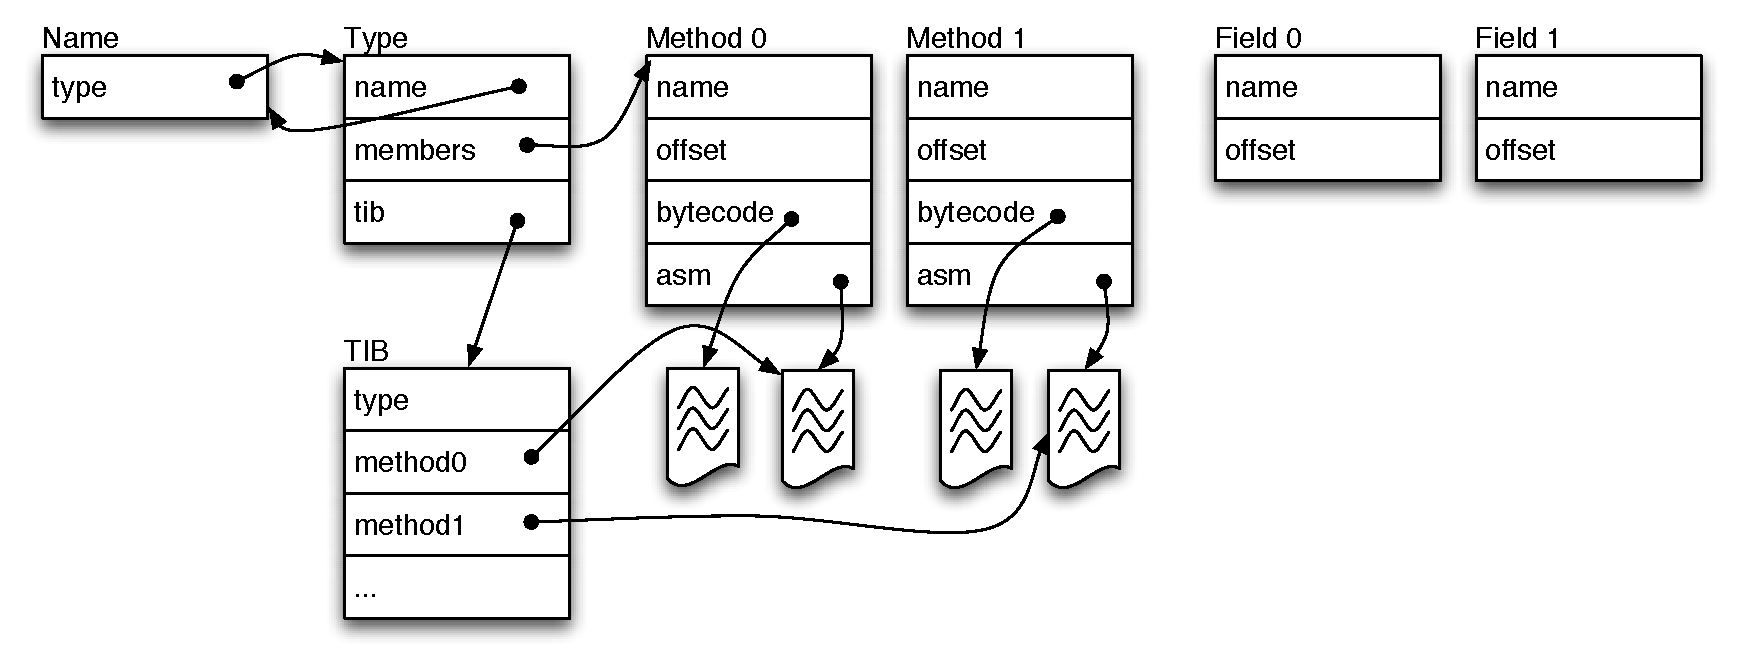
\includegraphics[scale=0.46]{100-images/vm-meta-data}
\hangcaption{\RVM meta-data schema for each class\label{fig:vm-meta-data}}
\VspaceFixForHangcaption
\end{figure}

\begin{figure}[t]
\centering
\includegraphics[scale=0.46]{100-images/vm-meta-data-updated-class}
\hangcaption{\RVM meta-data showing the old class name pointing to a newer
class after an update\label{fig:vm-meta-data-updated-classk}}
\VspaceFixForHangcaption
\end{figure}

\RVM represents classes with several internal data structures.
Figure~\ref{fig:vm-meta-data} shows the information \RVM associates
with a class.  Each class has an \VMClass meta-object that describes the
class. It points to other meta-objects that describe the class's method and
field types and offsets in an object instance.  The compiler and garbage
collector query this metadata. The compiler hard codes these offsets in
generated machine code when accessing fields and when calling methods.
These offsets are statically known when a class is loaded. \RVM and other
\VM{}s lay out fields and methods in \acfp{VMT} in such a way that a given
field or method has the same offset or slot in all subclasses. As explained
in Section~\ref{sec:dsu-view-of-changes}, in \acsp{VMT}, subclass methods
share the same slot as superclass methods they override. This sharing eases
\emph{dynamic dispatch} --- which method is called is decided at
runtime based on the object in hand. When a program invokes a method on an
object, the generated code indexes the object's \VMT at the correct offset
and jumps to the machine code. \RVM uses an array called the \acf{TIB} for
its \VMT. The first entry of the array points to the \VMClass meta-object
for that class. The garbage collector uses this entry to look up the type of a
particular object. The rest of the entries in the array serve as \VMT
slots.

For a class with only method body updates, all of the class's metadata is
the same in both the old and new versions. Therefore, \JV invalidates the
\TIB code entries for each replaced method, reads in the new method body
bytecode, and modifies the existing class metadata to refer to the
replacement methods' bytecode. The \JIT will compile the updated method
when the program next invokes it, after the update.

For a class with changed signature, the class's number, type, and order of
fields or methods may have changed, which in turn impacts the class's
metadata, including its \TIB. \JV modifies existing class metadata as
follows.  First, it changes the old class's metadata to use a modified
class name, e.g., metadata for class \User is renamed to \oUser in our
example update from Figure~\ref{fig:jes-string-emailaddress-example}
and~\ref{fig:jes-transformer-code}. At this point, it is as if {\tt class}
\User never existed. \JV reads in \User's class file as it normally does
and sets up metadata for the new version and updates its data structures
% (e.g., the Java Table of Contents for \static methods and fields)
to indicate that the newly-loaded class is now the up-to-date version.
Note that all \TIB entries for the newly-installed class are invalid, so
all methods in the class will be compiled on demand. \JV invalidates the
\TIB entries and other data structures for the old class so that they can
be garbage-collected.

Invalidating changed methods will impose overhead on the execution just
following the update when these methods are first \emph{base}-compiled and
then when they are progressively optimized at higher levels, if they
execute frequently. We could reduce this overhead somewhat by optimizing
new versions directly to their prior level of optimization. Updates to
method bodies however invalidate execution profiles and  without branch and
call frequencies, code quality would degrade. Thus, we believe it is better
to let the adaptive compiler work as it was intended. In any case, since
dynamic updates are relatively rare events, any added overhead due to
recompilation will be short-lived.

As mentioned in Section~\ref{sec:osr}, \JV uses on-stack replacement to
update active category~(2) methods. The VM triggers on-stack replacement
after the application resumes execution when callees of category~(2)
methods return. In order to resume execution, \JV must update data in the
heap. \JV initiates a full-heap garbage collection and transforms objects of
updated classes, which we get to next.

\subsection{Applying Transformers}
\label{sec:xformers}

We modify the \RVM semi-space copying collector~\cite{BCM:04,
Cheney:70}\index{semi-space copying collector} to update changed objects as
part of a collection. The collector traverses the heap, copies reachable
objects, and creates additional empty copies for all updated live objects. After collection, \JV walks through these
updated objects, runs their object transformers, and sets their fields
appropriately. We first examine \RVM's semi-space copying collector and the
tricolor abstraction~\cite{Dijkstra78, JL:96}\index{tricolor abstraction}
it maintains, and then present \JV's modifications.

In the tricolor abstraction, the \GC maintains colors for each object as it
performs a full-heap traversal to compute the transitive closure of
reachable objects. Objects have one of three colors: white objects are yet
to be visited; black objects have been visited and their immediate children
have been visited has well; grey objects have been visited but their
children might not have been visited. In this abstraction, collectors
maintain the invariant that no black object can point to
a white object. At the end of the traversal, there are no grey objects.
Objects that are unreachable are white and are freed by the
collector. Reachable objects are black and survive the collection.

\BCode[p]{0.75}
\begin{lstlisting}[frame=single, escapeinside={(*}{*)}]
function GC(roots):
   Q := empty
   for r in roots:
       r.color = GREY
       Q.add(r)
   while Q not empty:
       object = Q.pop()
       scanObject(object)

// precondition: object is GREY
function scanObject(object):(*\label{line:scan}*)
    for field in object:
        object.field = moveObject(object.field)
    object.color = BLACK

// precondition: object is either a forwarding
// pointer or a WHITE object. Either way,
// object resides in from space.
function moveObject(object):
    if object is real:
        copy = copyObject(object)
        copy.color = GREY
        Q.add(copy)
        object.FP = copy
        return copy
    if object is a forwarding pointer:
        return object.FP

// precondition: object is WHITE
function copyObject(object):
    copy = malloc() # in to space
    memcopy(copy, object)
    return copy
\end{lstlisting}
\ECode{Semi-space copying collector pseudo-code\label{fig:gc-code}}


The semi-space collector maintains the tricolor abstraction as follows. The
heap is divided into two spaces --- the currently active heap with all
objects, called the {\em from-space}, and an empty heap called {\em
to-space}. During the traversal, the collector copies reachable objects
from from-space to to-space and leaves unreachable ones in from-space. At
the end of collection, the entire from-space is reclaimed. Initially, all
objects in from-space are colored white. The traversal begins at {\em
roots}. The roots include statics, stack-allocated local variables, and
references in registers. The compiler generates a {\em stack map} at every
\VM safe point (a superset of \USD safe points).  The stack map enumerates
all register and local variables on the stack that reference heap objects.
The roots are not objects themselves, but are references to objects. The
roots reside outside the heap and are not copied. For the purposes of the
tricolor abstraction, the roots are initially colored gray.

The copying
collector walks through the list of grey objects and {\em scans} them (see
line~\ref{line:scan} in Figure~\ref{fig:gc-code}). Scanning an object
involves going through all reference fields of that object, moving the
referred objects over to to-space, and setting the field to the address
newly moved to. When moving an object, the collector leaves behind a {\em
forwarding pointer} in its place that points to the new location. This pointer
ensures that an object is moved only once and the forwarding pointer gives the
to-space address 
of the object. Later, if the collector encounters a
forwarding pointer when processing a reference, it sets the reference to
the value of the forwarding pointer.
Moving an object to to-space turns it
grey, while scanning an object makes it black. The fields of black objects
point to other objects in to-space, which are either grey or black.  The
fields of grey objects point to white objects (or forwarding pointers),
which are in from-space.
% \todo{You asked me to change the previous sentence to ``white objects or
% black objects that contain forwarding pointers''. Not sure if that is
% correct}
The traversal ends when there are no more grey
objects.

% We modify the \RVM semi-space copying collector \cite{BCM:04, Cheney:70} to update
% changed objects as part of a collection. The collector transforms old
% objects of an updated classes to conform to their new class signature and
% point to their new \acf{TIB}.  A semi-space copying collector normally
% works by traversing the pointer graph in the old heap (called
% \emph{from-space}) starting at the \emph{roots} and performing a transitive
% closure over the object graph, copying all objects it encounters to a new
% heap (called \emph{to-space}).  The roots include statics, stack-allocated
% local variables, and references in registers.  The compiler generates a
% \emph{stack map} at every VM safe point (a superset of DSU safe points).
% The stack map enumerates all register and local variables on the stack that
% reference heap objects.  When the collector first encounters an object, it
% copies it to to-space and then overwrites its header with a forwarding
% pointer to the new copy.  If the collector encounters a forwarded object
% later via another reference, it uses the forwarding pointer to redirect the
% reference to the new object. Forwarding pointers help the collector
% maintain the tricolor garbage collector invariant \cite{Dijkstra78, JL:96}
% and ensure each live object is copied exactly once, and all references to
% such an object point to the copy in to-space.

\BCode[p]{0.75}
\begin{lstlisting}[frame=single]
function moveObject(object):
    if object is real:
        copy = copyObject(object)
        copy.color = GREY
        Q.add(copy)
        if object.type.newVersion != null:
           newCopy = malloc()
           add newCopy to update log
           newCopy.type = object.type.newVersion
           // newCopy is currently empty
           object.FP = newCopy
           return newCopy
        else:
           object.FP = copy
           return copy
    if object is a forwarding pointer:
        return object.FP
\end{lstlisting}
\ECode{\JV's modification to \RVM's semi-space copying collector\label{fig:jvolve-gc-code}}


\begin{figure}[p]
\centering
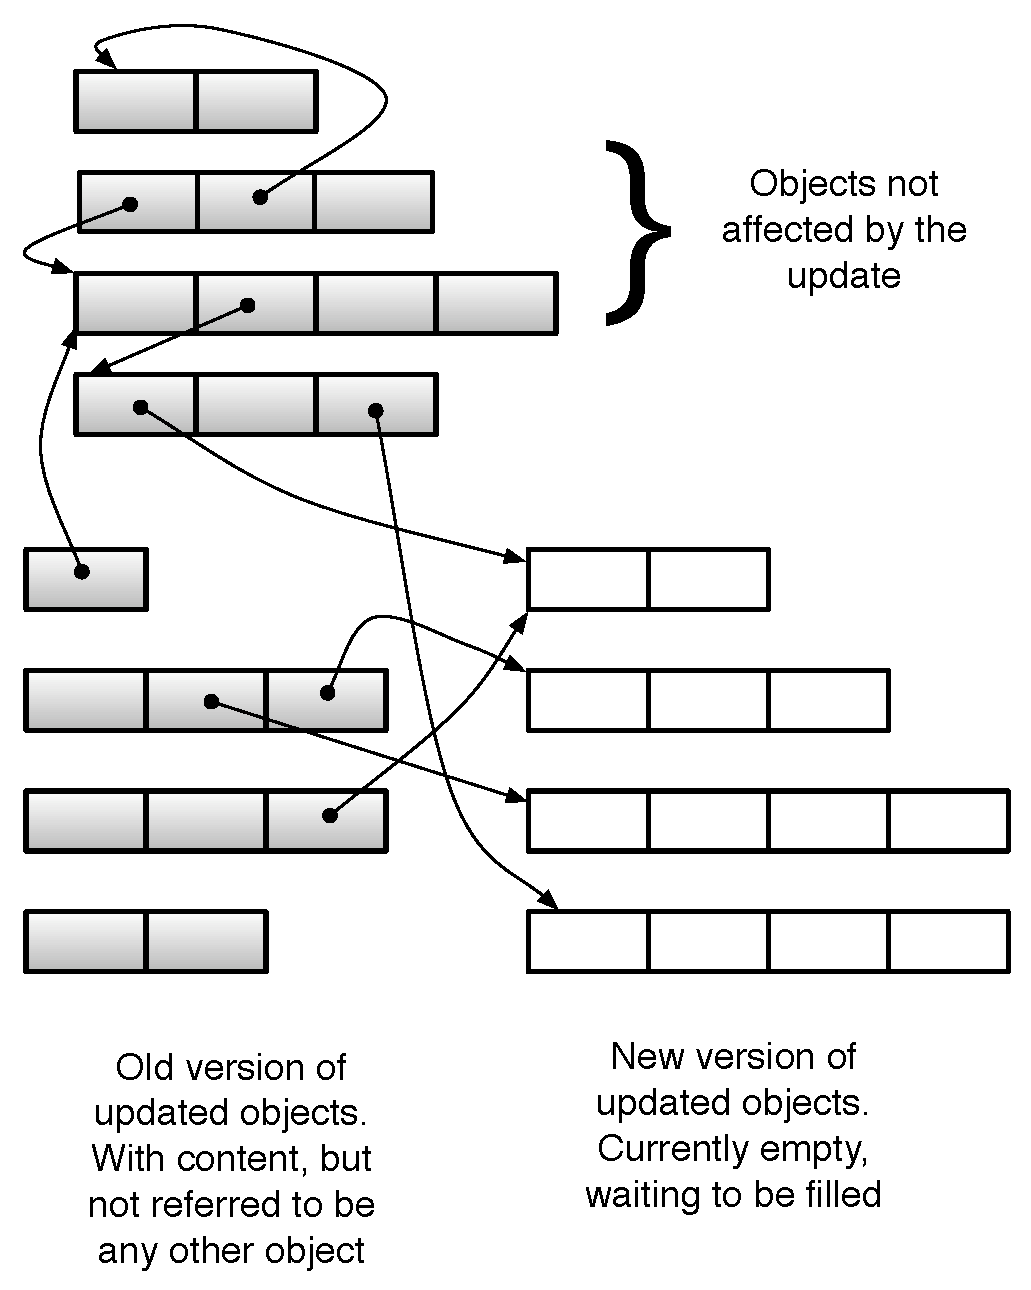
\includegraphics[scale=0.35]{100-images/to-space-after-gc}
\caption{A view of the \emph{to} semi-space immediately after garbage
collection\label{fig:to-space-after-gc}}
\end{figure}

\JV's modified collector works in much the same way as the regular
semi-space collector just described. As shown in
Figure~\ref{fig:jvolve-gc-code}, it differs in how it handles objects whose
class signature has changed.  In this case, it allocates a copy of the old
object \emph{and} an \emph{empty} new object according to the new class
definition, which may
have a different size compared to the old one. The collector initializes
the new object to point to the \acf{TIB}\iTIB of the new type, and installs the
forwarding pointer in from-space to this new version.  Next, the collector
stores a pair of pointers in its \emph{update log}, one to the copy of the
old object and one to the new object.  The collector continues scanning the
old copy. The key fact to note is that because forwarding pointers point to
the empty new copy of the object, references to updated types all point to
these empty objects.  Figure~\ref{fig:to-space-after-gc} illustrates this
situation. The old version of updated objects are filled with content while
references point to empty new versions of these objects.

After the collection completes, \JV adds another phase. It
first executes transformers for all
classes and then for all objects. 
%MWH: either order does not work equally well; both are wrong, really, but
%the current order is less likely to be wrong. See long e-mail exchange
%with %Suriya a while back.  We don't really handle this case correctly
%right now, so better to say little.
\JV goes through the update log and invokes the object transformer,
passing the old and new object pair as arguments. Recall from
Section~\ref{subsec:transformers} that the \JO functions receive an object
of the old version and an object of the new version as parameters. These
parameters come from the update log, with the old object filled with
content and the new object empty waiting to be filled by the transformer
function. Once \JV processes all object pairs, the log is deleted, making
the  duplicate old versions unreachable.
As Figure~\ref{fig:to-space-after-gc} shows, old version objects are
unreachable as no references point to them, and the next garbage collection
cycle will free them. While we did not do so in our implementation, we
could put these objects in a special space and reclaim the space
immediately after the update. We now look at two simple updates to
illustrate how \JV applies object transformers.

\begin{figure}[t]
\centering
\includegraphics[scale=0.7]{100-images/gcupdate}
\caption{Running object transformers following garbage collection}
\label{fig:gc-example}
\end{figure}

\paragraph{Example 1.} Figure~\ref{fig:gc-example} illustrates a part of
the heap at the end of the GC phase while applying the update from
Figure~\ref{fig:jes-transformer-code} (forwarding pointers are not shown).
On the
left is a depiction of part of the heap prior to the update.  It shows a
\User object whose fields point to various other elided objects.
After the copying phase, all of the old reachable objects are duplicated in
to-space.  The transformation log points to the new version of \User
(which is initially empty) and the duplicate of the old version, both of
which are in to-space.  The transformer function can safely copy fields of
the \FROM object. The figure shows that after running the transformer
function, the new version's {\tt username} field points to the same object
as before, and the new version's {\tt forwardAddresses} field points to a
new array of new {\tt EmailAddress} objects.
The {\tt EmailAddress} constructor called from within the
transformer function initialized these objects by referring to the old
e-mail {\tt String} values and assigning fields to point to substrings of
the given {\tt String}.

\begin{figure}[t]
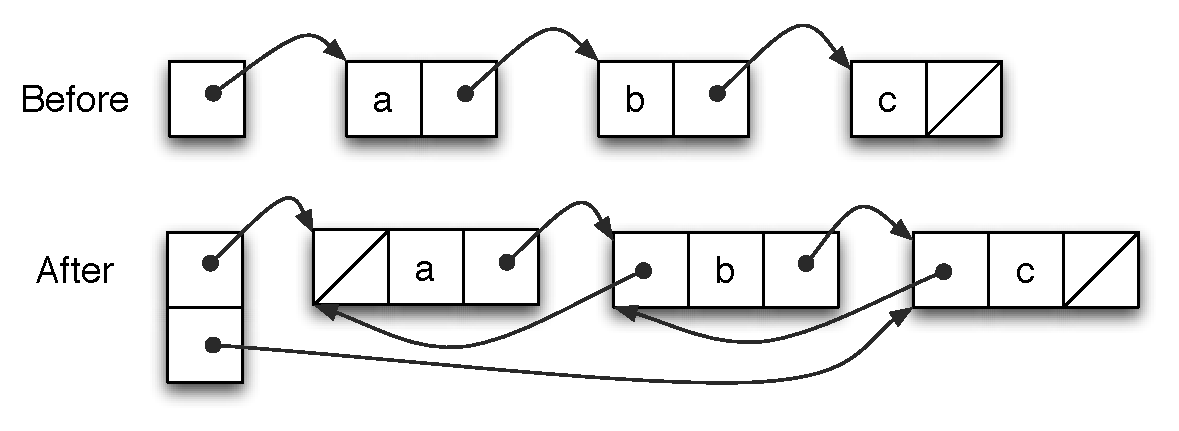
\includegraphics[scale=0.7]{100-images/linked-lists-without-gc}
\hangcaption{A look at the structure of an example linked list before and after the update
\label{fig:before-after-singly-doubly}}
\VspaceFixForHangcaption
\end{figure}

\begin{figure}[p]
\lstset{frame=single}
\begin{center}
\begin{tabular}{@{}c@{\hspace{0.07\textwidth}}c@{}}
\begin{minipage}{0.42\textwidth}
\begin{lstlisting}[title={Old version code}]
public class LinkedList {
  class Node {
    Node next;
    int data;
  }
  private Node head;
}
\end{lstlisting}
\end{minipage} &
\begin{minipage}{0.42\textwidth}
\begin{lstlisting}[title={New version code}]
public class LinkedList {
  class Node {
    Node prev;
    Node next;
    int data;
  }
  private Node head;
  private Node tail;
}
\end{lstlisting}
\end{minipage}
\end{tabular} \\[2ex]
\begin{minipage}{0.9\textwidth}
\begin{lstlisting}[frame=single,title={Stub classes for the old version}]
public class r0_LinkedList {
  public LinkedList.Node head;
  public class Node {
    public LinkedList.Node next;
    public int data;
  }
}
\end{lstlisting}
\end{minipage} \\[2ex]
\begin{minipage}{0.9\textwidth}
\begin{lstlisting}[frame=single,title={Default \UPT-generated transformer}]
public class JvolveTransformers {
  public static void jvolveObject(
      LinkedList.Node to, r0_LinkedList.Node from) {
    to.prev = null; // no such field in from
    to.next = from.next;
    to.data = from.data;
  }
  public static void jvolveClass(LinkedList.Node unused) {}
  public static void jvolveObject(
      LinkedList to, r0_LinkedList from) {
    to.head = from.head;
    to.tail = null; // no such field in from
  }
  public static void jvolveClass(LinkedList unused) {}
}
\end{lstlisting}
\end{minipage}
\end{center} 
\vspace*{-2ex}
% 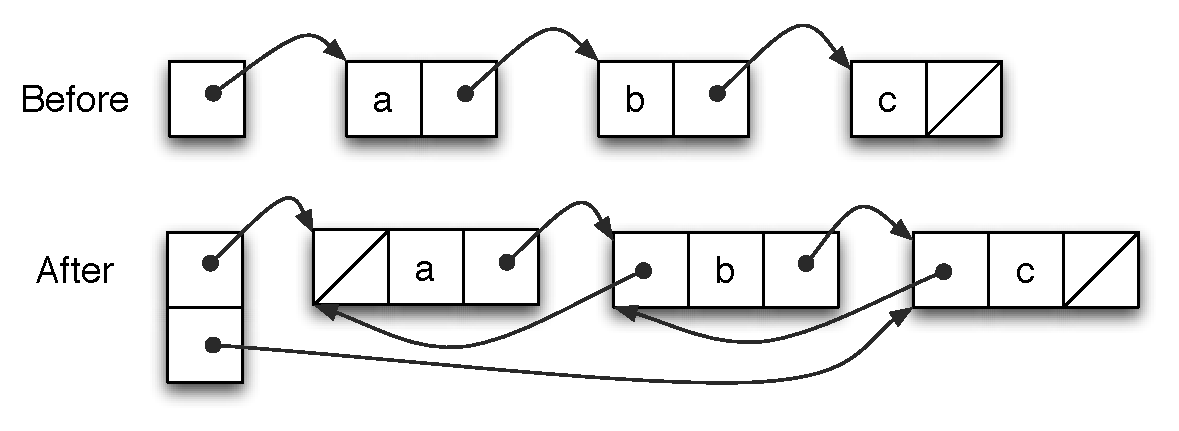
\includegraphics[scale=0.7]{100-images/linked-lists-without-gc}
\caption{An update that goes from a singly-linked to a doubly-linked list
\label{fig:singly-doubly}}
\lstset{frame=none}
\end{figure}


\paragraph{Example 2.}
We explore our object transformation\index{object transformer} model
by looking at another example.
Figure~\ref{fig:before-after-singly-doubly} shows an example linked list
before and after the update. In this example, a singly-linked list in the
old version becomes a doubly-linked list in the new.
Figure~\ref{fig:singly-doubly} shows the code for the old and new versions,
and stub classes and default transformers generated by the \acf{UPT}.
The update involves two classes with
signature changes: {\tt LinkedList} which adds a {\tt tail} field, and
{\tt Node} which adds a {\tt prev} field. The object transformers must
set these additional fields appropriately to create a doubly-linked list
out of a singly-linked one. The \JO functions generated by default will
correctly copy the {\tt data} and {\tt next} fields for each node in the
linked-list and correctly set {\tt head} to point to the start of the list.
We modify {\tt Node}'s transformer to set each node's {\tt next} node's
{\tt prev} field to point back to itself, i.e., {\tt from.next.prev =
from}.
Setting the {\tt tail} of the list to point to the last node is trickier.
We need some way to traverse the list to get to the end. At the time we
traverse the list, not all nodes might have been transformed. In order to
support this update, \JV provides a way for the programmer to request that
an object be transformed on-demand as the programmer traverses the list to
retrieve the {\tt tail} element of the list.  Section~\ref{sec:transformer-model}
explores this example in more detail and presents alternative object
transformation models.


\section{Conclusion}
We presented a detailed view of the \JV Virtual Machine. In the next
chapter we look at \JV's state transformer model and a novel way to
automatically generate state transformers.
